
\section[Problématique]{Position du problème et objectifs du stage}	
\noindent
\shadowbox{\begin{minipage}{\textwidth}
		\textbf{Résumé :} Le problème est de déterminer si un drone est capable de remplir une mission donnée, à partir d'une description formelle de la mission et d'un modèle de la dynamique du vol du drone. La méthode mise en œuvre implique des aspects de planification de commande, ainsi que de l'analyse de stabilité, et surtout l'intégration de ces outils. L'objectif est d'automatiser cette analyse le plus possible.
	\end{minipage}}
	
Dans le cadre de ce stage nous limiterons notre étude au problème longitudinal, c'est à dire que notre aéronef évoluera dans un espace 2D (distance et hauteur). Ceci nous permettra d'éprouver notre démarche sur un problème simple, puis par la suite d'étudier la faisabilité de notre démarche sur des déplacements longitudinaux et latéraux.

Les objectifs du stage sont multiples, tout d'abord il faut être capable de représenter mathématiquement un aéronef ayant des changements de modes de fonctionnement intrinsèques. Pour cela la démarche proposée est d'utiliser le formalisme des automates hybrides en considérant que chaque état de l'automate représente un mode de fonctionnement de l'aéronef (modélisé par un espace d'état linéaire).

Une fois que ce travail de modélisation de l'aéronef est effectué, il s'agit d'être capable de définir un environnement de mission et la mission, ceci dans le but de pouvoir planifier les commandes à appliquer à notre aéronef afin qu'il réussisse la mission. Tout ceci doit s'effectuer en garantissant la stabilité de l'aéronef.

Il est également à noter que ces travaux sont un préambule à différents projets futurs portant sur la planification des systèmes hybrides, nous devons déterminer les approches, outils, méthodes qui semblent être les plus pertinents pour résoudre ce type de problème.

L'environnement de la mission, c'est à dire le monde dans lequel l'aéronef va évoluer, peut se représenter sous la forme d'une coupe verticale de l'espace avec des zones interdites et des points de départ et d'arrivée. De plus la prise en compte des contraintes de stabilité de l'aéronef doit permettre d'éviter des scénarios dangereux, un exemple est présenté sur la figure \ref{fig:scenario} : 
%La zone rouge représente un nuage, la verte un couloir de navigation interdit et les bleu et jaune des montagnes. Les points de départ et d'arrivé sont également représenté.
\begin{figure}[!h]
	\centering	
	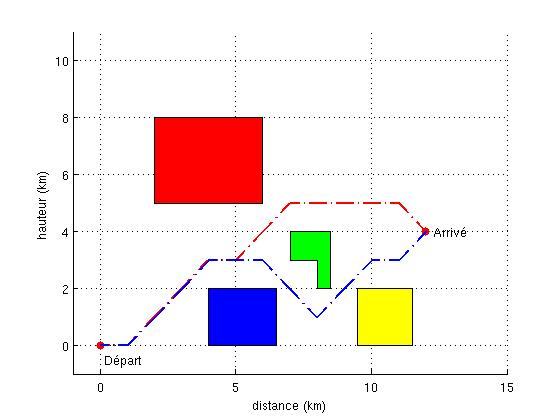
\includegraphics[scale=0.6]{images/scenario2.jpg}
	\caption{Environnement d'une mission}
	\label{fig:scenario}
\end{figure}

\pagebreak
Le scénario rouge semble respecter les contraintes de l'aéronef, en effet nous ne voyons pas de changement d'angle d'attaque trop élevé, en revanche, le scénario bleu présente un changement beaucoup trop brusque pour l'avion. Notre démarche doit donc permettre de fournir un scénario du type rouge.

%Nous faisons l'hypothèse que l'aéronef possède différentes lois de pilotage (monter, descendre, maintien, etc), chacune étant modélisée par un espace d'état linéaire (continu ou discret). L'interaction et les changements de loi de pilotage sont intrinsèques à l'aéronef et peuvent être représentés par un automate hybride.

Notre objectif est de proposer une démarche et des outils permettant la prise en compte d'un environnement, d'une mission et d'un aéronef présentant une dynamique hybride. La démarche doit être assez flexible et automatisée que possible, cela dans le but d'être appliquée à différents types d'aéronef et de mission.

Même si dans un premier temps l'exemple indiqué présente des aspects discrets limités qui peuvent être résolus manuellement, nous étudions des méthodes permettant de gérer des modèles dont la dynamique discrète est complexe (beaucoup d'obstacles, de points de passage, plusieurs avions/vols disponibles, etc...).

% comme présenté sur la figure \ref{exempleGraphe}.
%
%	\begin{figure}[!h]		
%		\centering	
%		\begin{tikzpicture}[->,>=stealth',shorten >=1pt,auto,node distance=2.8cm,
%		semithick,every text node part/.style={align=center}]
%		\tikzstyle{every state}=[fill=white,draw=black,text=black]
%		
%		
%		\node   (A)   at (2,1)  {};
%		\node[state]    (B)  at (3,0)     {mode 1 \\ maintien};
%		\draw[<-] (B) to[bend right] (A)  ;
%		
%		\node[state]    (C)   at (1,-3)     {mode 2 \\ monter};
%		\node[state]    (D)   at (5,-3)     {mode 3 \\ descendre};
%		
%		\path 
%		(B) edge [bend left=10] node {}   (C)		
%		(B) edge [bend right=10] node {}   (D)
%		
%		(C) edge [bend left=10] node {}   (B)		
%		(C) edge [bend left=10] node {}   (D)	
%		
%		(D) edge [bend left=10] node {}  (C)	
%		(D) edge [bend right=10] node {}  (B);		
%		\end{tikzpicture} 
%		\caption{Exemple d'automate hybride avec 3 lois de pilotage}
%		\label{exempleGraphe}
%	\end{figure}

%Une fois que nous avons le modèle de l'aéronef et que l'environnement de mission est établi, nous devons générer un plan répondant à la mission. Il faut s'assurer que ce plan ne va pas introduire d'instabilité sur l'engin. 

%Par exemple, sur la figure \ref{scenario} nous pouvons voir deux trajets répondant à la mission. Mais le trajet en bleu pose un problème car il imposerait des variations d'angle d'incidence entrainant un décrochage de l'aéronef.
%\begin{figure}[!h]
%\centering	
%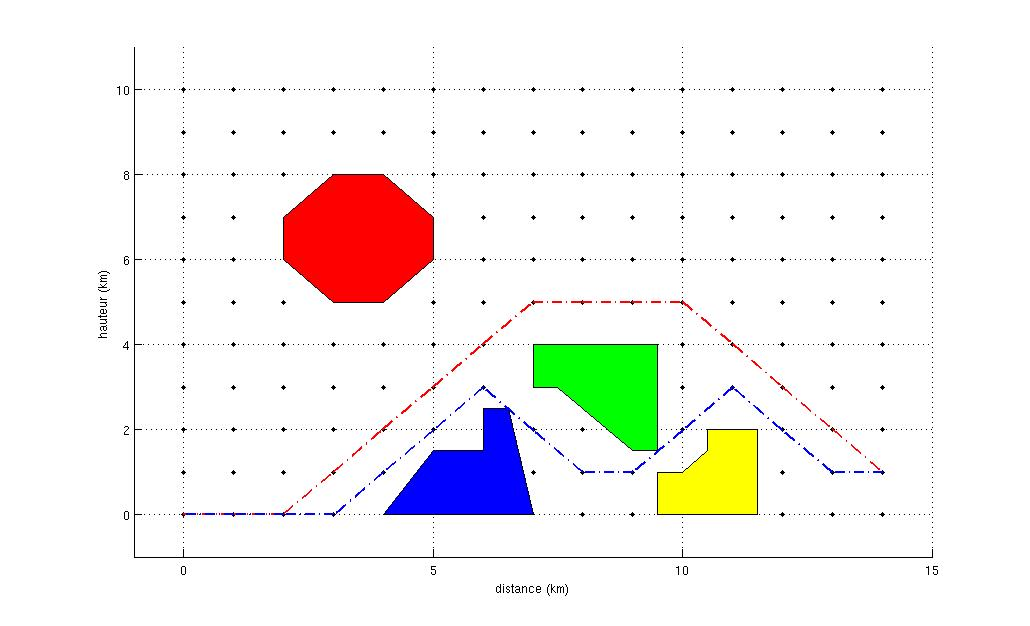
\includegraphics[scale=0.4]{images/scenario.jpg}
%\caption{Deux plans de mission (rouge : pas de soucis, bleu : décrochage possible)}
%\label{scenario}
%\end{figure}

